\section{迁移学习}

\subsection{概念及背景}

\begin{frame}{当前章节}
    \tableofcontents[currentsection, currentsubsection]
\end{frame}

\begin{frame}{迁移学习背景:大数据 大模型}
    \begin{columns}
        \column{0.5\textwidth}
        理想情况: 
        
        大量数据, 标注样本 --> 优秀模型\\[0.5cm]

        现实情况: 
        
        绝大多数据无标注
        
        收集大量标注数据并从头训练, 耗时耗力 

        \column{0.5\textwidth}
        \begin{figure}
            \centering
            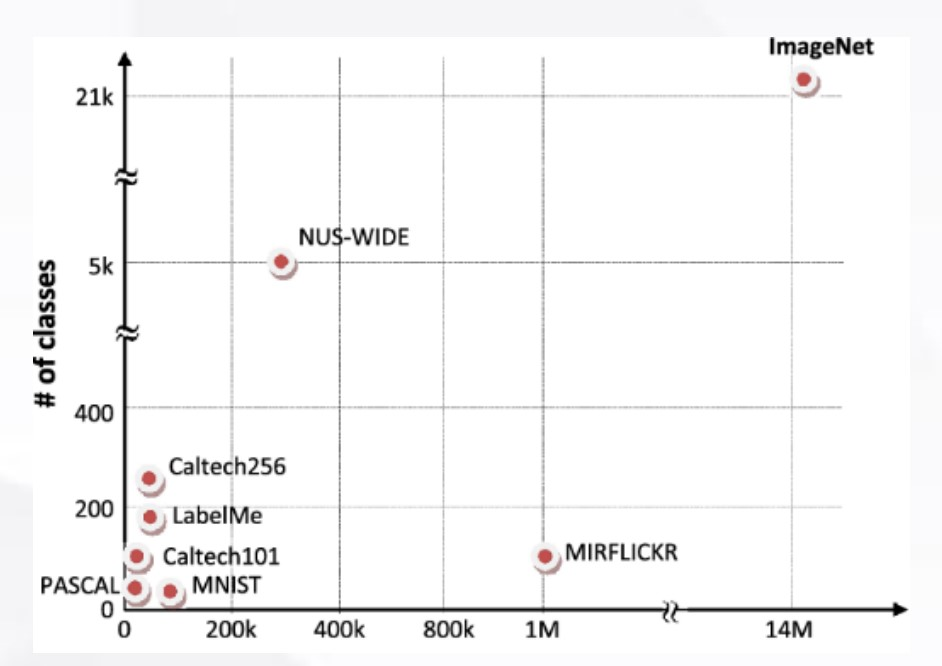
\includegraphics[width=\textwidth]{pic/pic01.jpg}
            \caption{数据集}
            \label{fig:01}
        \end{figure}

    \end{columns}
    
    
\end{frame}

\begin{frame}{迁移学习思想}
    利用辅助领域(源域)已有知识, 快速构建待学习领域(目标域)模型

    核心思想:
    \begin{itemize}
        \item 找到不同任务的相关性
        \item 举一反三, 利用已有大数据, 预训练模型完成自己任务
        \item 但不用``东施效颦''(负迁移)
    \end{itemize}

    \begin{columns}
        \column{0.5\textwidth}
        \begin{figure}
            \centering
            
\includegraphics[height=1.5cm]{pic/pic02.jpg}
            \label{fig:02}
        \end{figure}

        \column{0.5\textwidth}
        \begin{figure}
            \centering
            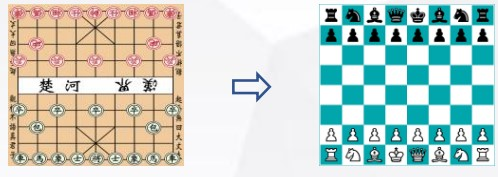
\includegraphics[height=1.5cm]{pic/pic03.jpg}
            \label{fig:03}
        \end{figure}
    \end{columns}
\end{frame}

\begin{frame}{迁移学习定义}
    给定源域$D_{s}=\{X_{i},y_{i}\}_{i=1}^{N_{s}}$, 和目标域$D_{t}=\{X_{j},y_{j}\}_{j=1}^{N_{t}}$, 其中$x\in \mathcal{X}, y\in \mathcal{Y}$. 迁移学习的目标是当以下三种情形:\\[0.5cm]
    \begin{enumerate}
        \item 特征空间不同, $\mathcal{X}_{s} \neq \mathcal{X}_{t}$
        \item 标签空间不同, $\mathcal{Y}_{s} \neq \mathcal{Y}_{t}$
        \item 特征和类别空间均相同, 概率分布不同, 即$P_{s}(x,y)\neq P_{t}(x,y)$
    \end{enumerate}
    \hspace{1cm}\\[0.5cm]
    至少有一种成立时, 利用源域数据去学习一个目标域上的预测函数$f:x_{t} \to y_{t}$, 使得$f$在目标域上拥有最小的预测误差:

    \begin{equation*}
        f^{\star} = arg \min \limits_{f} E_{\{x,y\}\in D_{t}} \epsilon(f(x),y)
    \end{equation*}
\end{frame}


\begin{frame}{为什么要迁移学习}
    \begin{columns}

        \column{0.5\textwidth}
        \begin{figure}
            \centering
            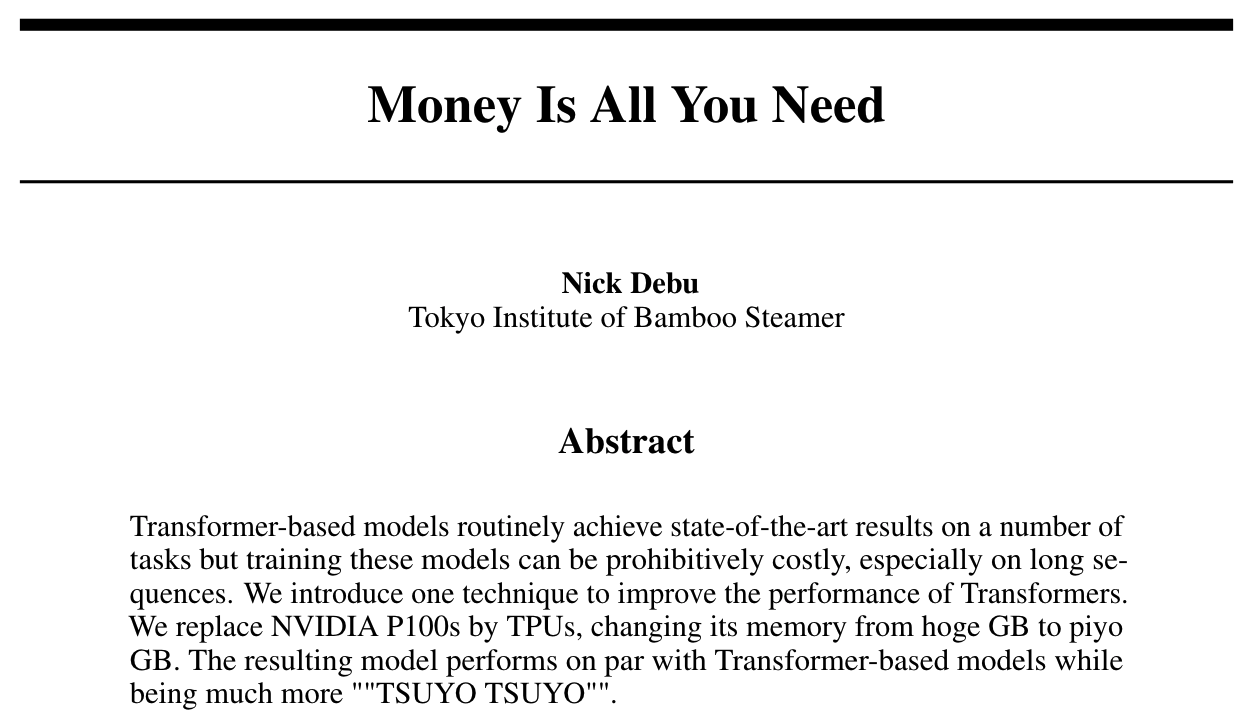
\includegraphics[width=\textwidth]{pic/pic04.png}
            \caption{Money is all we need}
            \label{fig:04}
        \end{figure}
        
        \column{0.5\textwidth}
        \begin{itemize}
            \item 大数据与少标注
            \item 大数据与弱计算能力
            \item 有限数据与模型泛化能力
        \end{itemize}

    \end{columns}
\end{frame}

\begin{frame}{区别与联系}
    迁移学习与传统机器学习区别联系:
    \begin{itemize}
        \item 数据分布: 训练测试数据服从不同分布
        \item 数据标注: 不需要足够的数据标注
        \item 模型: 模型可以在不同任务之间迁移
    \end{itemize}

    多任务(multi-task)和领域自适应(Domain adaptation)都属于迁移学习的范畴内. 
    
\end{frame}


\subsection{迁移学习分类}


\begin{frame}{当前章节}
    \tableofcontents[currentsection, currentsubsection]
\end{frame}

\begin{frame}{迁移学习分类}
    \begin{figure}
        \centering
        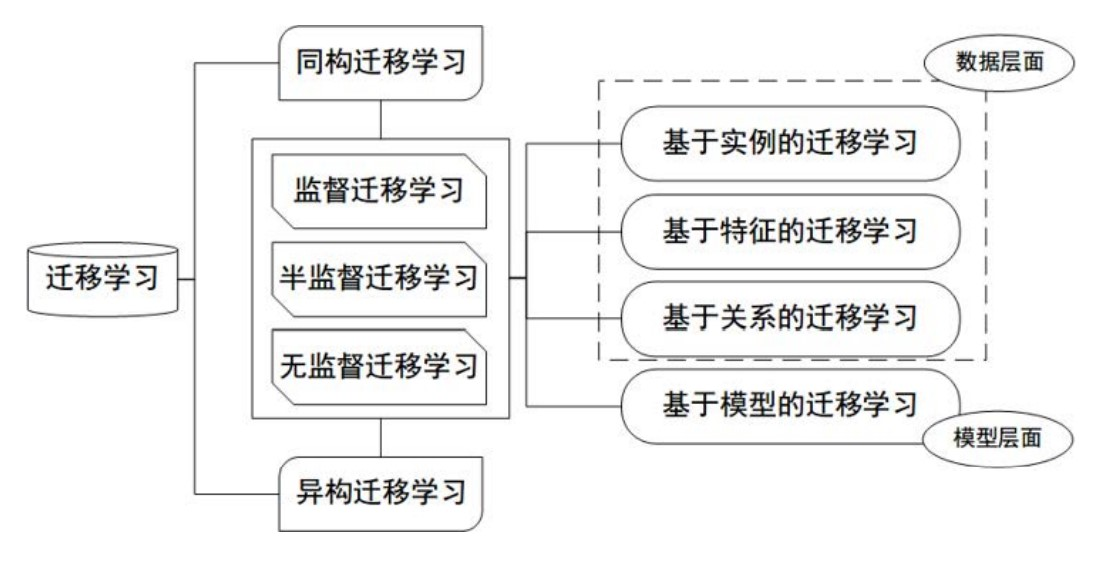
\includegraphics[width=\textwidth]{pic/pic05.jpg}
        \caption{迁移学习分类}
        \label{fig:05}
    \end{figure}
\end{frame}



\subsection{深度迁移学习}

\begin{frame}{当前章节}
    \tableofcontents[currentsection, currentsubsection]
\end{frame}

\begin{frame}{DL 可迁移性}
    \begin{figure}
        \centering
        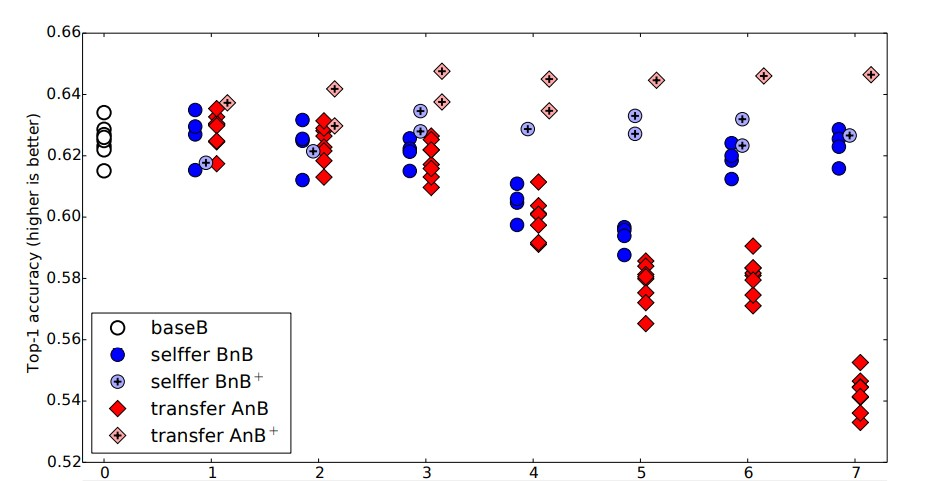
\includegraphics[width=\textwidth]{pic/pic0201.jpg}
        \caption{How transferable are features in deep neural networks?}
        \label{fig:06}
    \end{figure}
    
\end{frame}

\begin{frame}{Finetune}
    预训练模型并不完全适用于自己的任务:
    \begin{itemize}
        \item 数据分布不同
        \item 任务复杂度不同
    \end{itemize}

    \hspace{1cm}\\[0.5cm]
    Finetune的优势在于:
    \begin{itemize}
        \item 不需要对新任务从头开始训练网络, 节省了时间成本
        \item 预训练模型在大数据集中训练, 无形中扩大了我们的训练数据, 可使模型泛化性更强
        \item 相比重新设计网络, Finetune实现简单
    \end{itemize}
\end{frame}

\begin{frame}{深度网络自适应}

    \begin{columns}

        \column{0.5\textwidth}
        自适应使源域和目标域数据在高维特征空间分布更接近
        \begin{itemize}
            \item 哪些层自适应
            \item 适应层有多少层
            \item 采用什么样的自适应方法
        \end{itemize}
        
        \column{0.5\textwidth}
        \begin{figure}
            \centering
            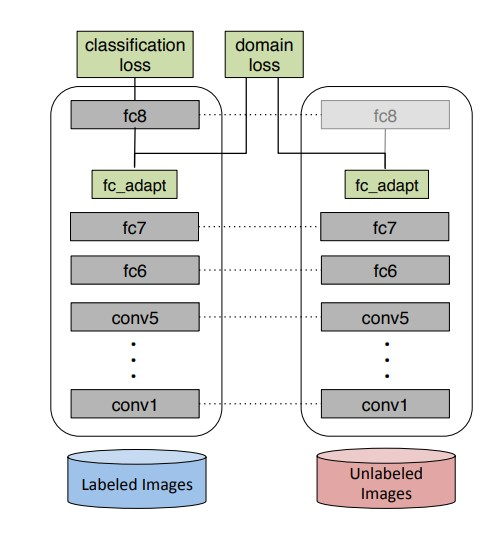
\includegraphics[height=0.7\textheight]{pic/pic0202.jpg}
            \caption{Adaptation Layer}
            \label{fig:07}
        \end{figure}

    \end{columns}
\end{frame}

\begin{frame}{深度网络对抗迁移}
    借鉴GAN对抗思想
    \begin{itemize}
        \item DANN(Domain-Adversarial NN)
        \item DSN(Domain Separation Networks)
    \end{itemize}
\end{frame}

\begin{frame}{Domain-Adversarial Neural Networks}
    \begin{figure}
        \centering
        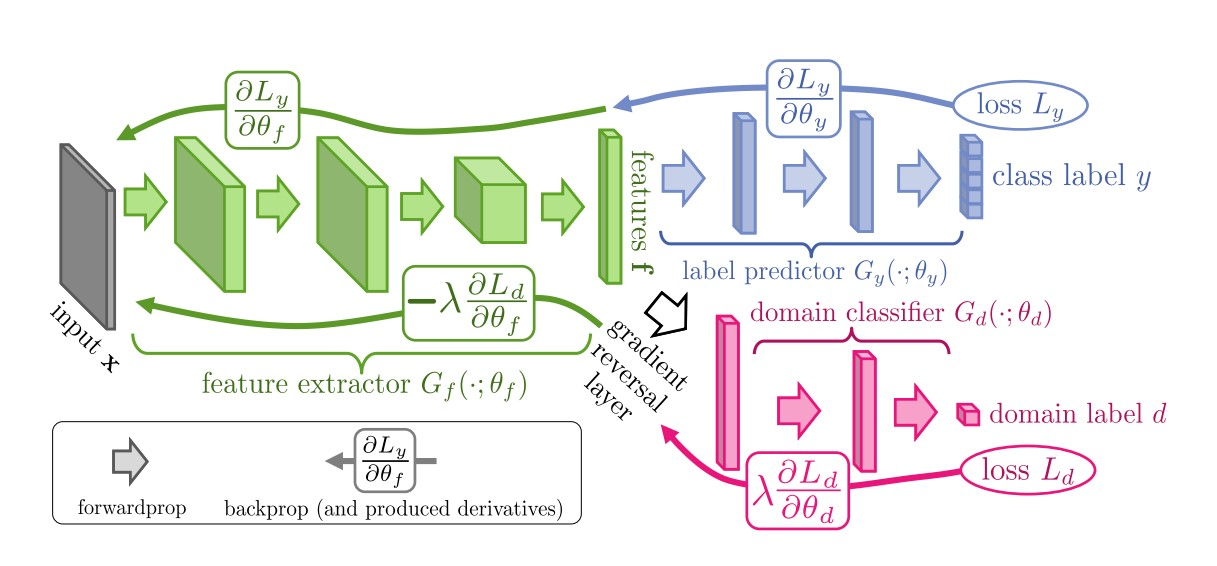
\includegraphics[width=\textwidth]{pic/pic0203.jpg}
        \caption{Domain-Adversarial Neural Networks}
        \label{fig:08}
    \end{figure}
\end{frame}

\begin{frame}{Domain Separation Networks}
    \begin{figure}
        \centering
        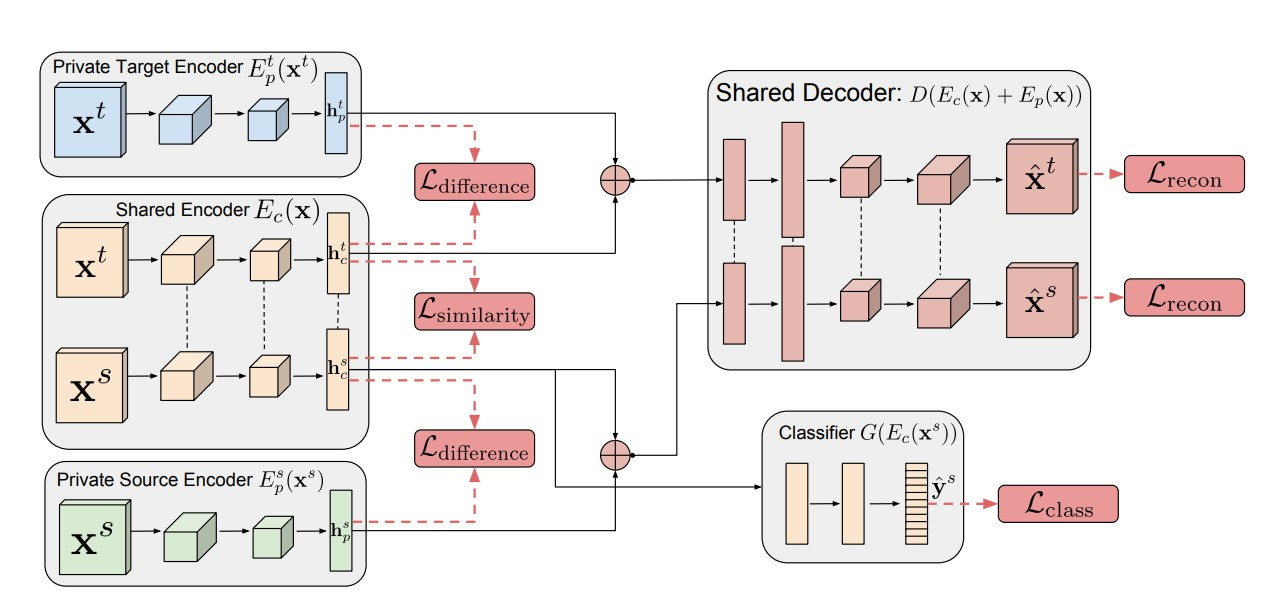
\includegraphics[width=\textwidth]{pic/pic0204.jpg}
        \caption{Domain Separation Networks}
        \label{fig:09}
    \end{figure}
\end{frame}